\clearpage
\section{Physical channel7: ADC and integrators, 17 November 2026}
Both USB pairs moved8 to7 in the same5--8 fitting. Independent active/inhibited
bypass probes verified DAC0/1 at J8, DAC2/3 at J6 and normal selector map[0,1].
MCU1803, FPGA ff2f746c and power checks passed. The same frozen method/source
contracts as channel8 were matched; previous selected result IDs are unchanged.
No programming or clock changes, and no repetition of the completed5--8 timing,
monitor or internal-DAC scans.
\subsection{ADC transfer and adjacent bits: PASS}
Both banks were swept at257points from-1.2 to+1.2V differential,1V common mode,
with outputs0.4--1.6V. Every bit and all44adjacent-pair states were exercised.
\begin{center}\begin{tabular}{lrrr}\toprule
ADC & Gain(code/V) & Zero mean(code) & Template-removed RMS(code)\\\midrule
A & -1780.88 & 2174.111 & 0.558 \\
B & -1777.82 & 2165.762 & 0.554 \\
\bottomrule\end{tabular}\end{center}
\begin{center}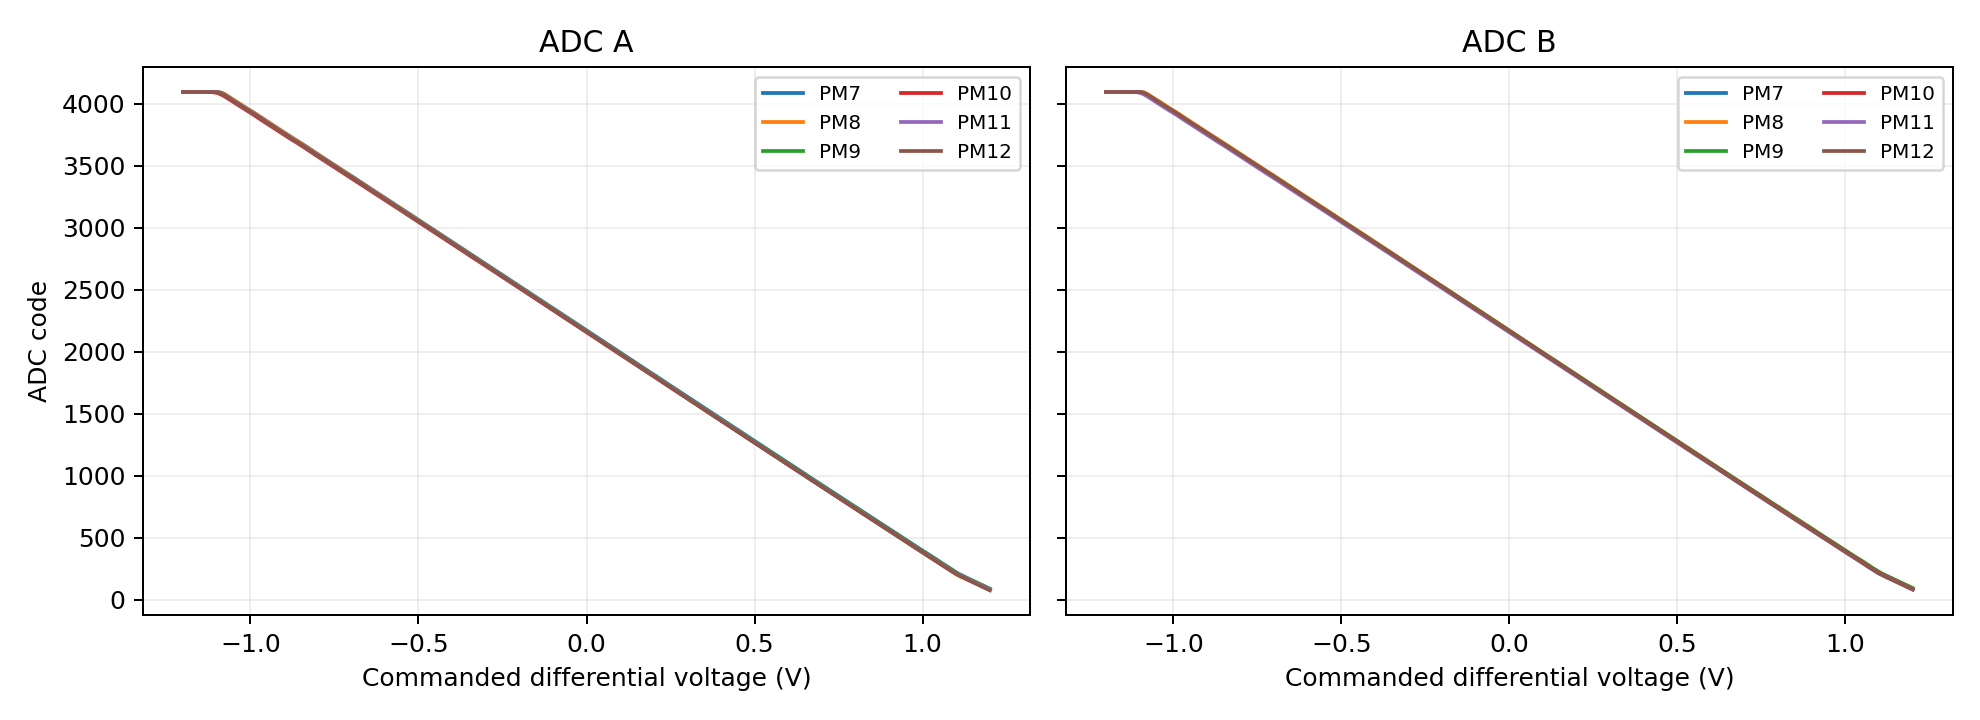
\includegraphics[width=\linewidth]{ch07-adc-dc-07-12.png}\end{center}
These are commanded-voltage, whole-chain observations. Template-removed RMS is
not intrinsic ADC noise or aperture jitter. Older10--12 use c7c42d28;7--9 use
ff2f746c with their separately recorded source contracts and capture conditions.
\subsection{Integrator balance and signed response: PASS}
Coarse13 and fine26points at0.4mV, followed by independent candidate returns
and plus/minus5mV controls, verified an unclipped signed zero crossing per bank.
\begin{center}\begin{tabular}{lrrr}\toprule
ADC & DAC2/DAC3(V) & Return change(code) & Gain(code/V)\\\midrule
A & 1.0268/2.0452 & +0.265 & -2683.0 \\
B & 1.0262/2.0458 & -0.285 & -2612.8 \\
\bottomrule\end{tabular}\end{center}
\begin{center}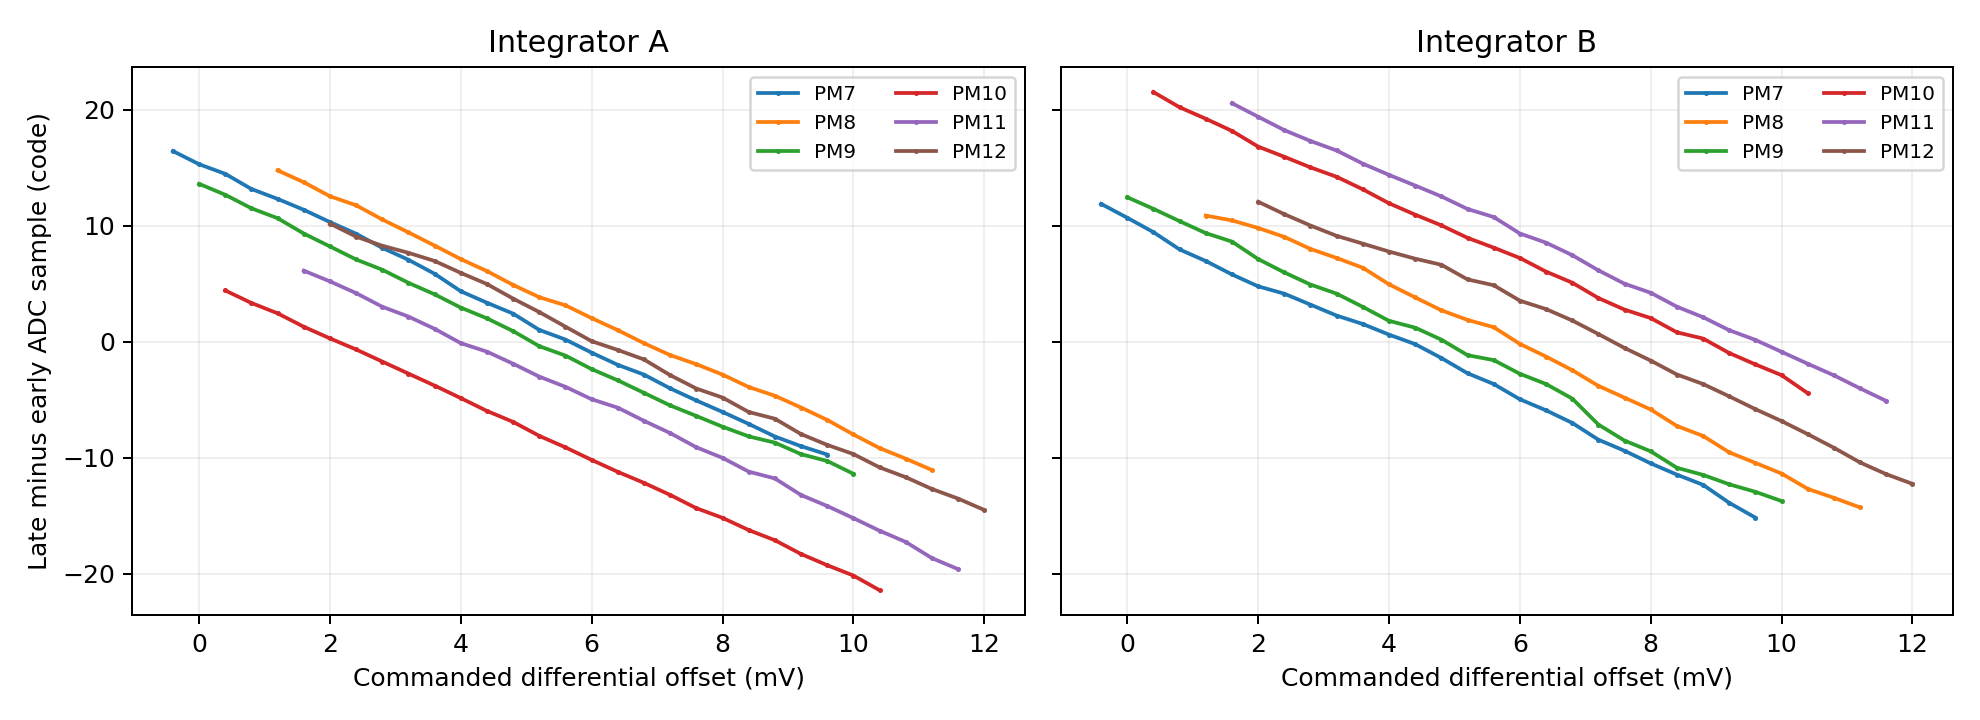
\includegraphics[width=\linewidth]{ch07-integrator-07-12.png}\end{center}
The sampled integration pair is waveform-derived, not independently gate-tagged.
Final DAC0/1 are1/1V; DAC2/3 use the shared measured compromise recorded in the
raw metadata. Channel7 amplifiers enabled, direct ADC bypass isolated, all
monitor muxes inhibited/TCA0. Other fitted channels were isolated at preflight.
Kasli outputs/directions unchanged; leases released. Analog7--12 observations
are now available;5--6 await their USB moves.

\subsection{Zero-input waveforms and FFT}
The selected zero-differential buffers for channels7--12 are compared below.
Capture origins are local, not synchronized between channels. FFT amplitudes
are one-sided RMS code per bin at nominal80.1574MS/s, not spectral density or
an intrinsic ADC aperture-jitter measurement.
\begin{center}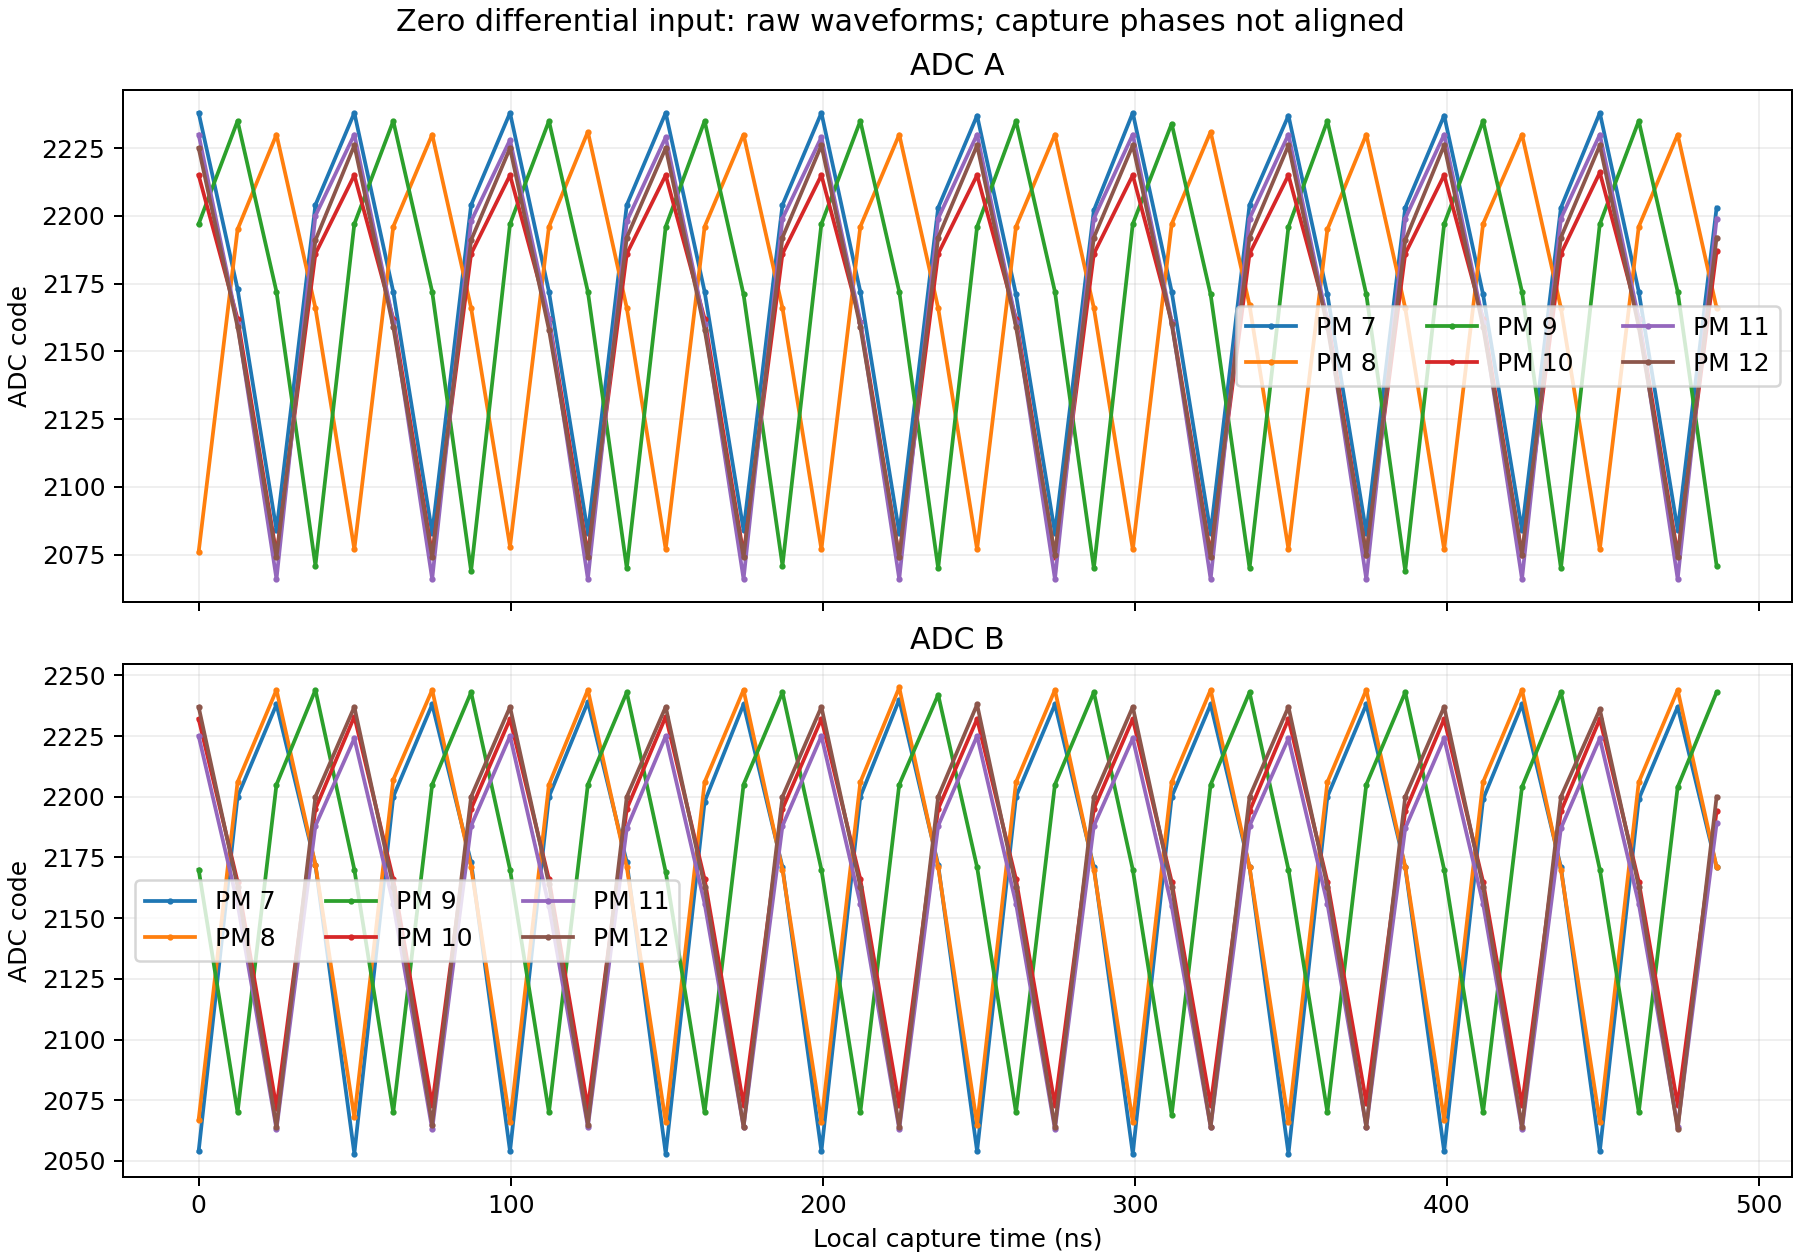
\includegraphics[width=\linewidth]{ch07-adc-zero-time.png}\end{center}
\begin{center}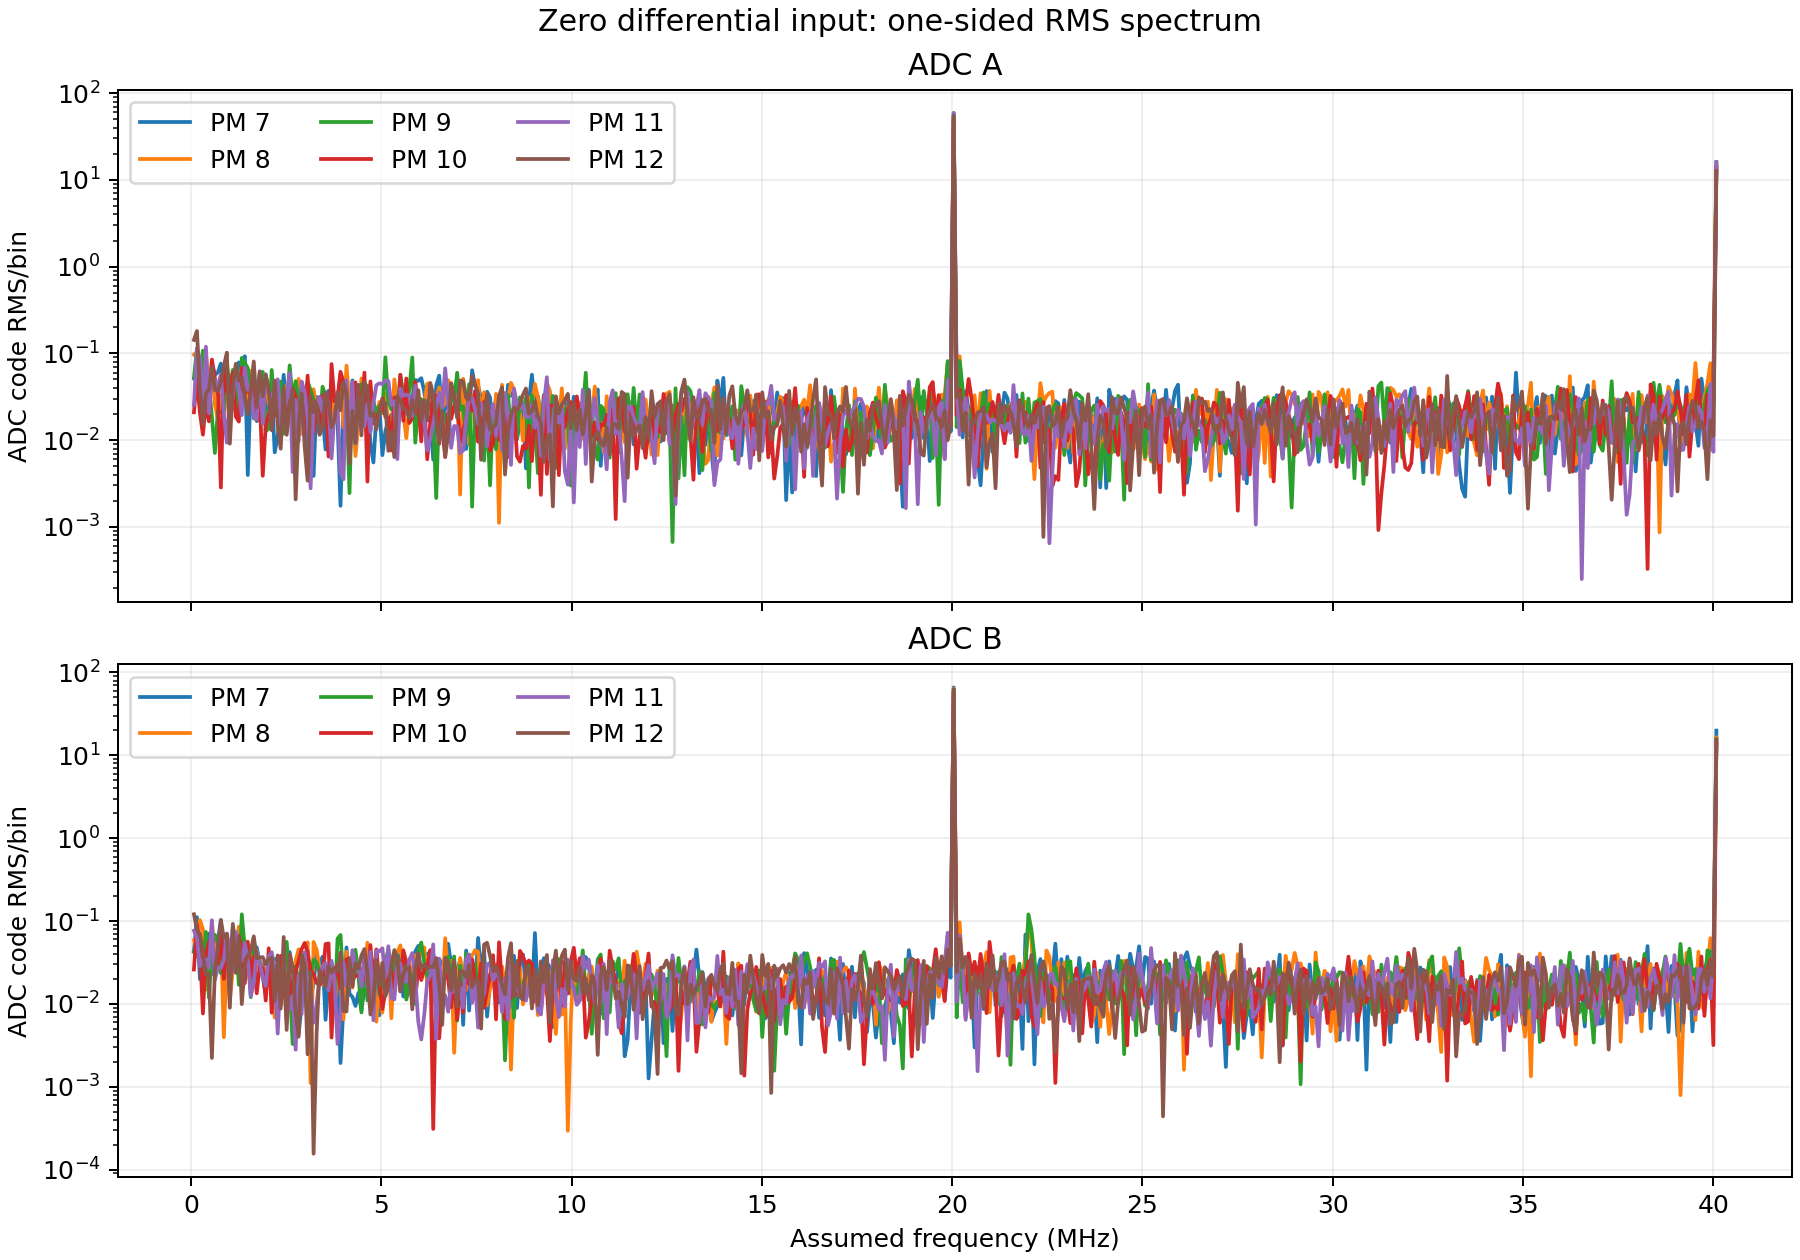
\includegraphics[width=\linewidth]{ch07-adc-zero-fft.png}\end{center}
